\section{Praxisbeispiel}\label{sec:praxisbeispiel}
Im Folgenden wird der Workflow mit \gls{dfl} näher betrachtet.
Anschließend werden verschiedenen Konfigurationen und Trainingsdauern verglichen.

\subsection{Laborumgebung}\label{subsec:laborumgebung}
Alle Deepfakes, wenn nicht anders genannt, werden auf folgender Hardware erstellt.\\[0.5cm]
\begin{tabular}{rl}
    CPU:& \texttt{AMD Ryzen 5 2600X}\\
    RAM:& \texttt{16GB DDR4 3000MHz}\\
    GPU:& \texttt{NVIDIA RTX 2070 (8GB GDDR6 VRAM)}\\
    OS:& \texttt{Windows 11}
\end{tabular}\\[0.5cm]

Ziel des Deepfakes ist das Gesicht von \gls{rdj} auf Prof. Volker Knoblauch in diesem \href{https://www.youtube.com/watch?v=rksMPlRSbQU}{Video} zu swappen,
sodass die Hochschule Aalen amerikanische Prominente auf ihrem Youtube-Kanal zeigen kann.

\subsection{Programmstruktur}\label{subsec:programmstruktur}
Nach der Installation von \gls{dfl} finden sich im entsprechenden Ordner eine Vielzahl von \texttt{.bat}-Dateien, sowie ein \texttt{\_internal}- und \texttt{workspace}-Ordner.
Die \texttt{.bat}-Dateien führen die im \texttt{\_internal}-Ordner abgelegten Scripte mit den entsprechenden Parametern aus.
Es wäre also möglich auf die Dateien zu verzichten und \gls{dfl} lediglich über eine Konsole auszuführen.
Alle Dateien, die während der Erstellung eines Deepfakes erstellt oder benötigt werden, werden im \texttt{workspace}-Ordner abgelegt.
Bei der Installation von \gls{dfl} werden Beispieldaten mit geladen.\\

Immer wieder finden sich die Bezeichnungen \texttt{src} und \texttt{dst}.
Diese referenzieren in \gls{dfl}:
\begin{itemize}
    \item \textbf{src (Source):} Das Gesicht, bzw. das zugehörige Videomaterial, das über das Zielgesicht gelegt werden soll.
    \item \textbf{dst (Destination):} Das Gesicht, bzw. das zugehöhrige Videomaterial, das ersetzt werden soll.
\end{itemize}

\subsection{Vorbereitung}\label{subsec:vorbereitung}
Bevor ein Deepfake erstellt werden kann, muss zuerst einmal geeignetes Ausgangsmaterial gesammelt werden.
Generell gilt, je besser das Trainingsmaterial, desto besser werden die Deepfakes.
Die Qualität des Ausgangsmaterials hängt von der Auflösung, der Belichtung, der Vielseitigkeit der Ausdrücke und der verschiedenen Aufnahmewinkeln (Fig. \ref{fig:head-angles-diagram}) ab.
Dabei gilt, je ähnlicher Source- und Destination-Material sind, desto überzeugender wird das Ergebnis.
\begin{figure}
    \center
    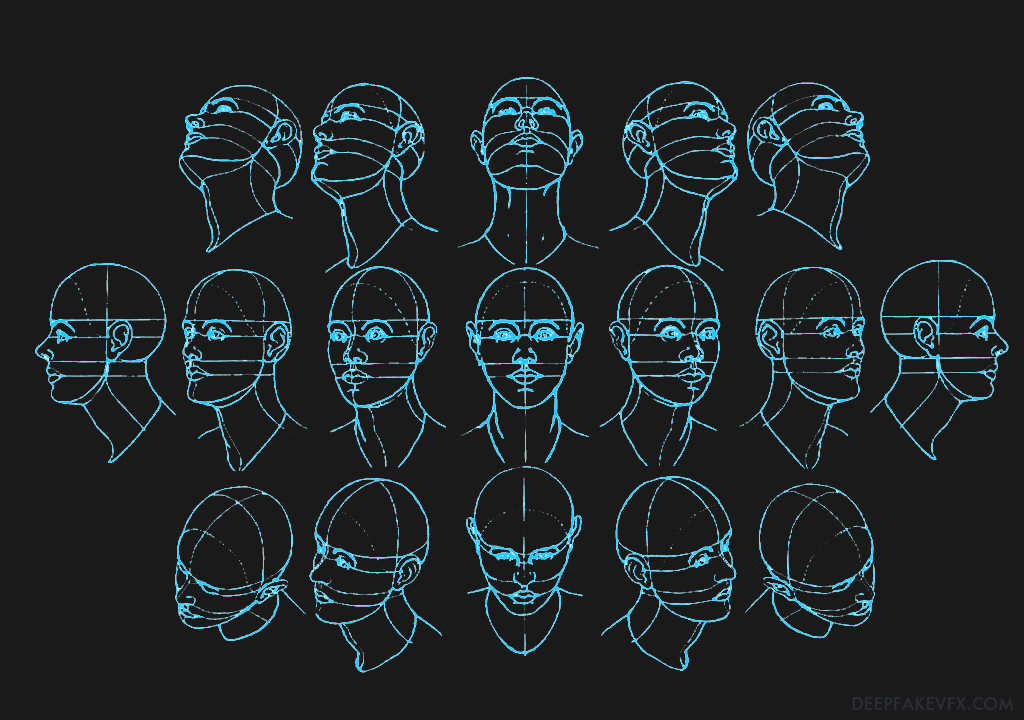
\includegraphics[width=0.5\textwidth]{Bilder/DFL/Human_Head_Angles_Diagram}
    \caption{Head Angles Diagram}
    \label{fig:head-angles-diagram}
\end{figure}

Ein Trainingsdatensatz sollte mehrere Hundert Bilder umfassen.
Je nach Resolution des trainierten Models sollten die Zahlen sogar in die Tausende gehen.\\[0.5cm]

Für den exemplarischen Deepfake dieser Arbeit, werden das mitgelieferte Standardvideo von \gls{rdj} als \texttt{Source} und das Interview von Prof. Dr. Harald Rieger und Prof. Volker Knoblauch als \texttt{Destination} verwendet.

